\documentclass[12pt,a4paper]{article}

\usepackage{minted}
\usepackage[T1]{fontenc}
\usepackage[export]{adjustbox}
\usepackage{graphicx}

\renewcommand*\contentsname{Spis treści}

\title{Stacja pogodowa oparta na mikrokontrolerze ESP32 z interfejsem użytkownika oraz API}
\author{Szymon Uglis}

\begin{document}

\begin{titlepage}
    \maketitle
\end{titlepage}

\tableofcontents{}
\pagebreak

\section{Wstęp}

Celem projektu jest utworzenie urządzenia do celów kolekcji danych pogodowych. 

Urządzenie, będzie udostępniało również interfejs programistyczny API REST, które będzie umożliwiało integracje oraz dalszy rozwój projektu 
(np. integracja z systemem home assitant czy innymi urządzeniami Internetu rzeczy (IoT))

\section{Opis rozwiązania tworzonego w ramach projektu}

\paragraph{Funkcje urządzenia:}
\begin{itemize}
    \item Pomiar oraz kalkulacja danych pogodowych na podstawie danych wejściowych z czujników
    \item Udostępnienie i agregacja danych w postaci strony www
    \item Udostępnienie interfejsu programistycznego REST 
\end{itemize}

\subsection{Wykorzystane technologie}
Do implemntacji systemu wbudowanego wykorzystane zostaną:
\begin{itemize}
    \item Język C do utworzenia oprogramowania mikrokontrolera
    \item Środowisko programistyczne Arduino Studio
    \item Język HTML oraz CSS do utworzenia interfejsu www
\end{itemize}

\subsection{Zastosowany mikrokontroler oraz czujniki} \label{list_of_components}

\begin{itemize}
    \item Mikrokontroler ESP-WROOM-32
    \item Czujnik natężenia światła - TSL25911
    \item Czujnik temperatury i wilgotności - DHT22
    \item Czujnik ciśnienia oraz temperatury - DPS310
\end{itemize}

\subsection{Opis 7W}

\subsubsection{Why: Dlaczego powstaje taki produkt?}
Urządzenie oraz aplikacja powstaje w celu zbioru oraz prezentacji danych pogodowych w formacie przyjaznym dla uzytkownika oraz w formacie, który
umożliwi integrację z innymi systemami.

\subsubsection{What: Co trzeba zrobić?}
Należy przygotować urządzenie umożliwiające kolekcję danych oraz ich udostępnianie oraz należy przygotować oprogramowanie, które będzie 
sterowało pracą urządzenia.

\subsubsection{When: Na kiedy trzeba zrobić?}

Wytwarzanie prototypu produktu zajmie 120 dni. Od 28.10.2023 do 28.02.2024.

\subsubsection{Who: Kto jest odpowiedzialny za poszczególne funkcje produktu?}

\begin{itemize}
    \item Klient
    \item Programista (1)
\end{itemize}

\subsubsection{Where: Gdzie znajdują sie ludzie związani z projektem?}
Wrocławska Akademia Biznesu w Naukach Stosowanych, ul. Aleksandra Ostrowskiego 22, 53-238 Wrocław

\subsubsection{How: Jak powstanie produkt i jak będą przebiegać prace?}

Zostanie skonstruowane urządzenie za pomocą komponentów wymienionych w punkcie \ref{list_of_components} oraz zostanie napisane 
oprogramowanie sterujące w języku C. Produkt będzie wytwarzany w metodologii waterfall.

\subsubsection{How: }

Wytwarzanie prototypu produktu zajmie 120 dni.

\subsection{Wymagania niefunkcyjne}

\begin{enumerate}
    \item Prostota instalacji urządzenia (maksymalnie 3 kroki od odpakowania do gotowego do działania urządzenia)
    \item Możliwość zasilenia za pomocą kabla typu USB-C
    \item Łatwość dostępu do danych dla końcowego użytkownika (strona www)
    \item Dokumentacja do połączenia z API programistycznym
    \item Możliwość aktualizacji oprogramowania urządzenia z minimalnym czasem przerwy w pracy
    \item Kompatybilność z każdym chipem ESP-32
    \item Strona www dla użytkownika stworzona w technologiach HTML, CSS oraz Javascript
    \item Interfejs programistyczny REST API zwraca dane w formacie JSON
\end{enumerate}

\subsection{Wymagania funkcyjne}

\begin{enumerate}
    \item Podłączenie urządzenia oraz pierwsza konfiguracja\\
    Opis: Podłączenie urządzenia do źródła zasilania, wyszukanie punktu wifi urządzenia, wpisanie dostępów do wifi docelowego\\
    Wejście: Urządzenie podłączone do zasilania, połączenie sie z punktem dostępowym urządzenia\\
    Wyjście: Urządzenie podłączy sie do podanej przez użytkownika sieci bezprzewodowej
    \item Wyświetlanie aktualnych danych z urządzenia\\
    Opis: Odwiedzenie strony www stworzonej przez urządzenie, odczytanie danych zebrnych przez urządzenie w formacie łatwo dostępnym dla
    użytkownika końcowego\\
    Wejście: Przejście na stronę internetową udostępnianą przez urządzenie\\
    Wyjście: Załadowana strona z aktualnymi danymi z urządzenia\\
    \item Wyświetlenie danych historycznych\\
    Opis: Odczyt danych historycznych zbieranych przez urządzenie\\
    Wejście: Bezpośrednie odwiedzenie strony www lub klikcięcie w przycisk nawigujacy do podstrony z historią ze strony głównej\\
    Wyjście: Załadowana strona z danymi historycznymi urządzenia\\
    \item Wyświetlenie strony z ustawieniami\\
    Opis: Odczyt oraz zmiana ustawień urządznia\\
    Wejście: Bezpośrednie odwiedzenie strony www lub klikcięcie w przycisk nawigujacy do podstrony z ustawieniami ze strony głównej\\
    Wyjście: Załadowana strona z ustawieniami urządzenia\\
    \item Eksport danych historycznych do pliku\\
    Opis: Możliwość eksportu danych historycznych zapisanych na urządzeniu do formatu json lub csv\\
    Wejście: Podanie zakresu dat do eksportu danych, wybranie formatu pliku w jakim ma być eksport zrealizowany\\
    Wyjście: Zostanie pobrany plik w wybranym formacie z danumi z wybranego zakresu\\
\end{enumerate}

\subsection{Przypadki użycia}

\begin{enumerate}
    \item Uruchomienie urządzenia w docelowej lokalizacji\\
    CEL: Uruchomienie urządzenia w celu zbioru danych pogodowych
    \begin{enumerate}
        \item Rozpakowanie urządzenia, podłączenie do zasilania
        \item Podłączenie sie sie do punktu dostępowego udostępnianego przez urządzenie w celu podłaczenia do sieci bezprzewodowej użytkownika
        \item Urządzenie podłączyło sie do podanej sieci bez przewodowej, jeśli nie to wróc do punktu b)
    \end{enumerate}
    \item Odczyt danych pogodowych\\
    CEL: Odczytanie aktualnyuch danych pogodowych zbieranych przez urządzenie
    \begin{enumerate}
        \item Odwiedzenie strony głównej urządzenia
    \end{enumerate}
    \item Odczyt danych historycznych\\
    CEL: Odczytanie historycznych danych pogodowych zbieranych przez urządzenie
    \begin{enumerate}
        \item Odwiedzenie strony głównej urządzenia
        \item Przejście za pomocą łącza na stronie głównej o nazwie "Dane Historyczne", które przekieruje na podstronę z danymi historycznymi
    \end{enumerate}
    \item Eksport danych historycznych\\
    CEL: Eksport danych historycznych zebranych przez urządzenie do pliku
    \begin{enumerate}
        \item Odwiedzenie podstrony z danymi historycznymi
        \item W sekcji "Eksport" wybranie zakresu dat w jakich ma eksport być wykonany oraz formatu pliku do jakiego eksport ma być utworzony
        \item Kliknięcie w przycisk "Eksportuj" w sekcji "Eksport"
        \item Przeglądarka pobierze plik z wyeksportowanymi danymi
    \end{enumerate}
    \item Odczyt aktualnych ustawień urządzenia\\
    CEL: Odczytanie aktualnych ustawień komponentów urządzenia
    \begin{enumerate}
        \item Odwiedzenie strony głównej urządzenia
        \item Przejście za pomocą łącza na stronie głównej o nazwie "Ustawienia", które przekieruje na podstronę z danymi historycznymi
    \end{enumerate}
\end{enumerate}

\section{Opis ryzyka}

\subsection{Potencjalne zagrożenia}

\begin{enumerate}
    \item Niedotrzymanie terminu\\
    Prawodopodobieństwo: małe\\
    Istnotność: katastrofalna\\
    Przyczyny:
    \begin{itemize}
        \item Słaba koordynacja prac
        \item Nieprzewidziany problem techniczny
    \end{itemize}
    Skutki:
    \begin{itemize}
        \item Zapłata kar umownych
        \item Strata klienta
    \end{itemize}

    \item Wyniki testów poniżej dopuszczalnej normy jakości\\
    Prawodopodobieństwo: małe\\
    Istnotność: katastrofalna\\
    Przyczyny:
    \begin{itemize}
        \item Nieprzewidziany problem techniczny
        \item Zbyt małe doświadcznie zespołu
    \end{itemize}
    Skutki:
    \begin{itemize}
        \item Opóźnienie kolejnego etapu prac
        \item Możliwa konieczność przygotowania części systemu od początku
    \end{itemize}

    \item Niedostateczne spełneinie oczekiwań klienta\\
    Prawodopodobieństwo: małe\\
    Istnotność: katastrofalna\\
    Przyczyny:
    \begin{itemize}
        \item Brak lub słaba komunikacja z klientem
        \item Złe lub niedostateczne zrozumienie wymagań klienta
    \end{itemize}
    Skutki:
    \begin{itemize}
        \item Opóźnienie kolejnego etapu prac
        \item Możliwa konieczność przygotowania części systemu od początku
    \end{itemize}

    \item Niska wydajność przygotowanego systemu\\
    Prawodopodobieństwo: małe\\
    Istnotność: katastrofalna\\
    Przyczyny:
    \begin{itemize}
        \item Dobranie komponentów z zbyt małej wydajności
        \item Kiepska optymalizacji kodu
    \end{itemize}
    Skutki:
    \begin{itemize}
        \item Wolne działanie systemu - długie ładowanie stron, długie czasy eksportów danych
    \end{itemize}
\end{enumerate}


\subsection{Plany awaryjne}

\begin{enumerate}
    \item Niedotrzymanie terminu
        \begin{enumerate}
            \item Zwiększenie liczby godzin pracy
            \item Zatrudnienie dodatkowych osób
        \end{enumerate}
    \item Wyniki testów poniżej dopuszczalnej normy jakości
        \begin{enumerate}
            \item Dokładna analiza modułów sprawiających najwięcej błędów
        \end{enumerate}
    \item Niedostateczne spełnienie oczekiwań klienta
        \begin{enumerate}
            \item Analiza wszystkich wcześniejszych ustaleń i dokumentacji projetkowej
            \item Weryfikacja poprawności systemu do ustaleń z klientem
            \item Wyznaczenie dodatkowego planu działania w przypadku potrzeby poprawy systemu
        \end{enumerate}
    \item Niedostateczne spełnienie oczekiwań klienta
        \begin{enumerate}
            \item Analiza wszystkich wcześniejszych ustaleń i dokumentacji projetkowej
            \item Weryfikacja poprawności systemu do ustaleń z klientem
            \item Wyznaczenie dodatkowego planu działania w przypadku potrzeby poprawy systemu
        \end{enumerate}
    \item Wolniejsze działanie aplikacji niż zamierzone
        \begin{enumerate}
            \item Analiza problemów wydajnościowych systemy
            \item Wyznaczenie dodatkowego planu działania w przypadku potrzeby poprawy systemu
        \end{enumerate}
\end{enumerate}

\section{Diagramy}

\subsection{Diagram przypadków użycia}
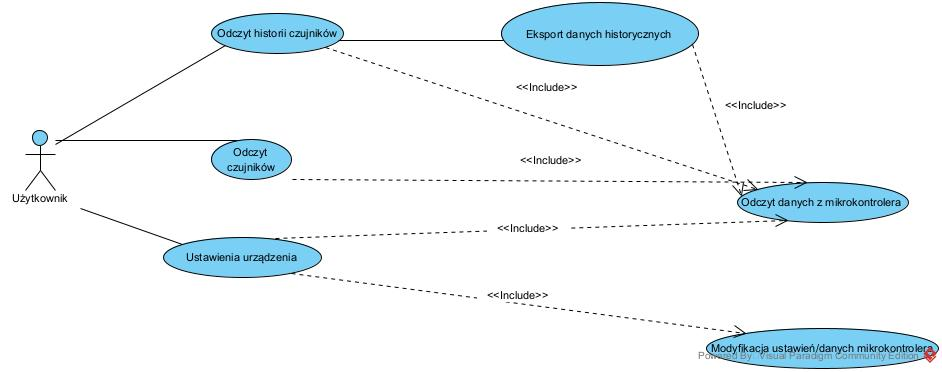
\includegraphics[width=\textwidth, center]{use-case-diagram-1.jpg}

\subsection{Diagram sekwencji}
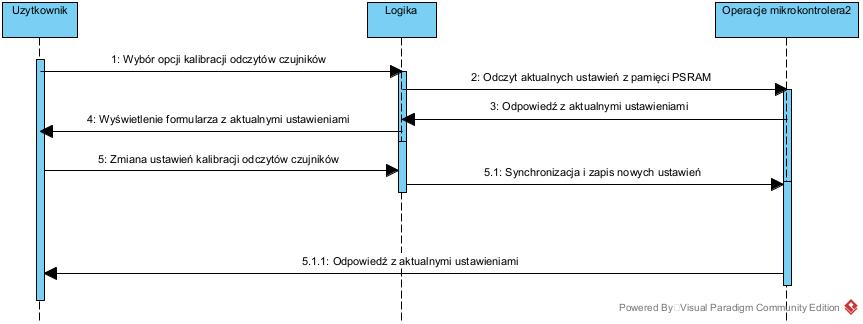
\includegraphics[width=\textwidth, center]{sequence-diagram-2.jpg}

\subsection{Diagram aktywności}
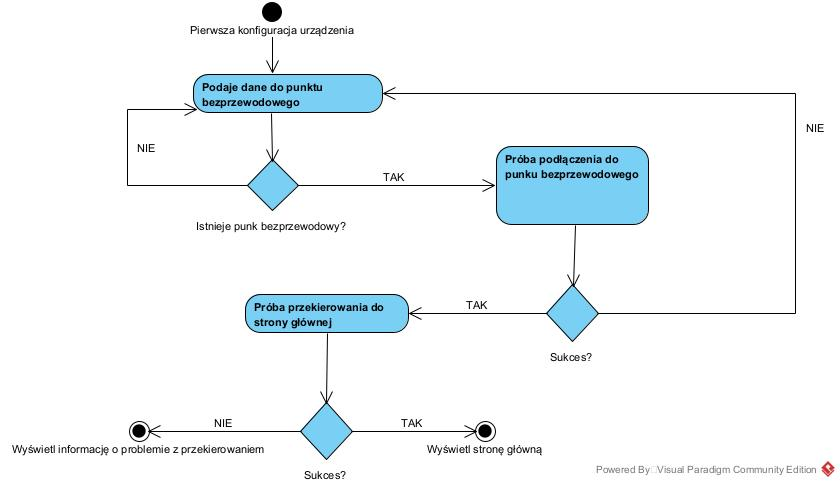
\includegraphics[width=\textwidth, center]{activity-diagram.jpg}

\subsection{Diagram klas}

Ze względu, że projekt jest systemem wbudowanym na diagrame klas zostały zaprezentowane jakie
funkcje są wykonywane.

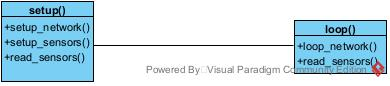
\includegraphics[width=\textwidth, center]{class-diagram.jpg}

\subsection{Diagram wdrożenia}
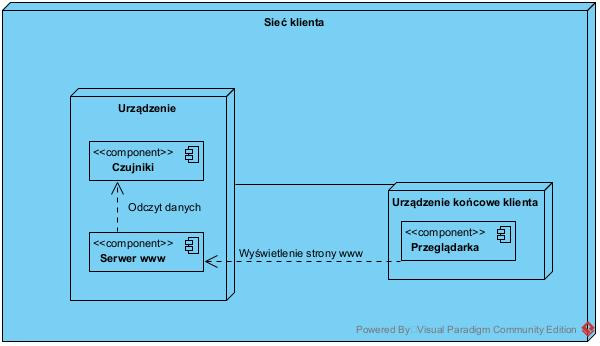
\includegraphics[width=\textwidth, center]{deployment-diagram.jpg}

\subsection{Wykres Gantta}
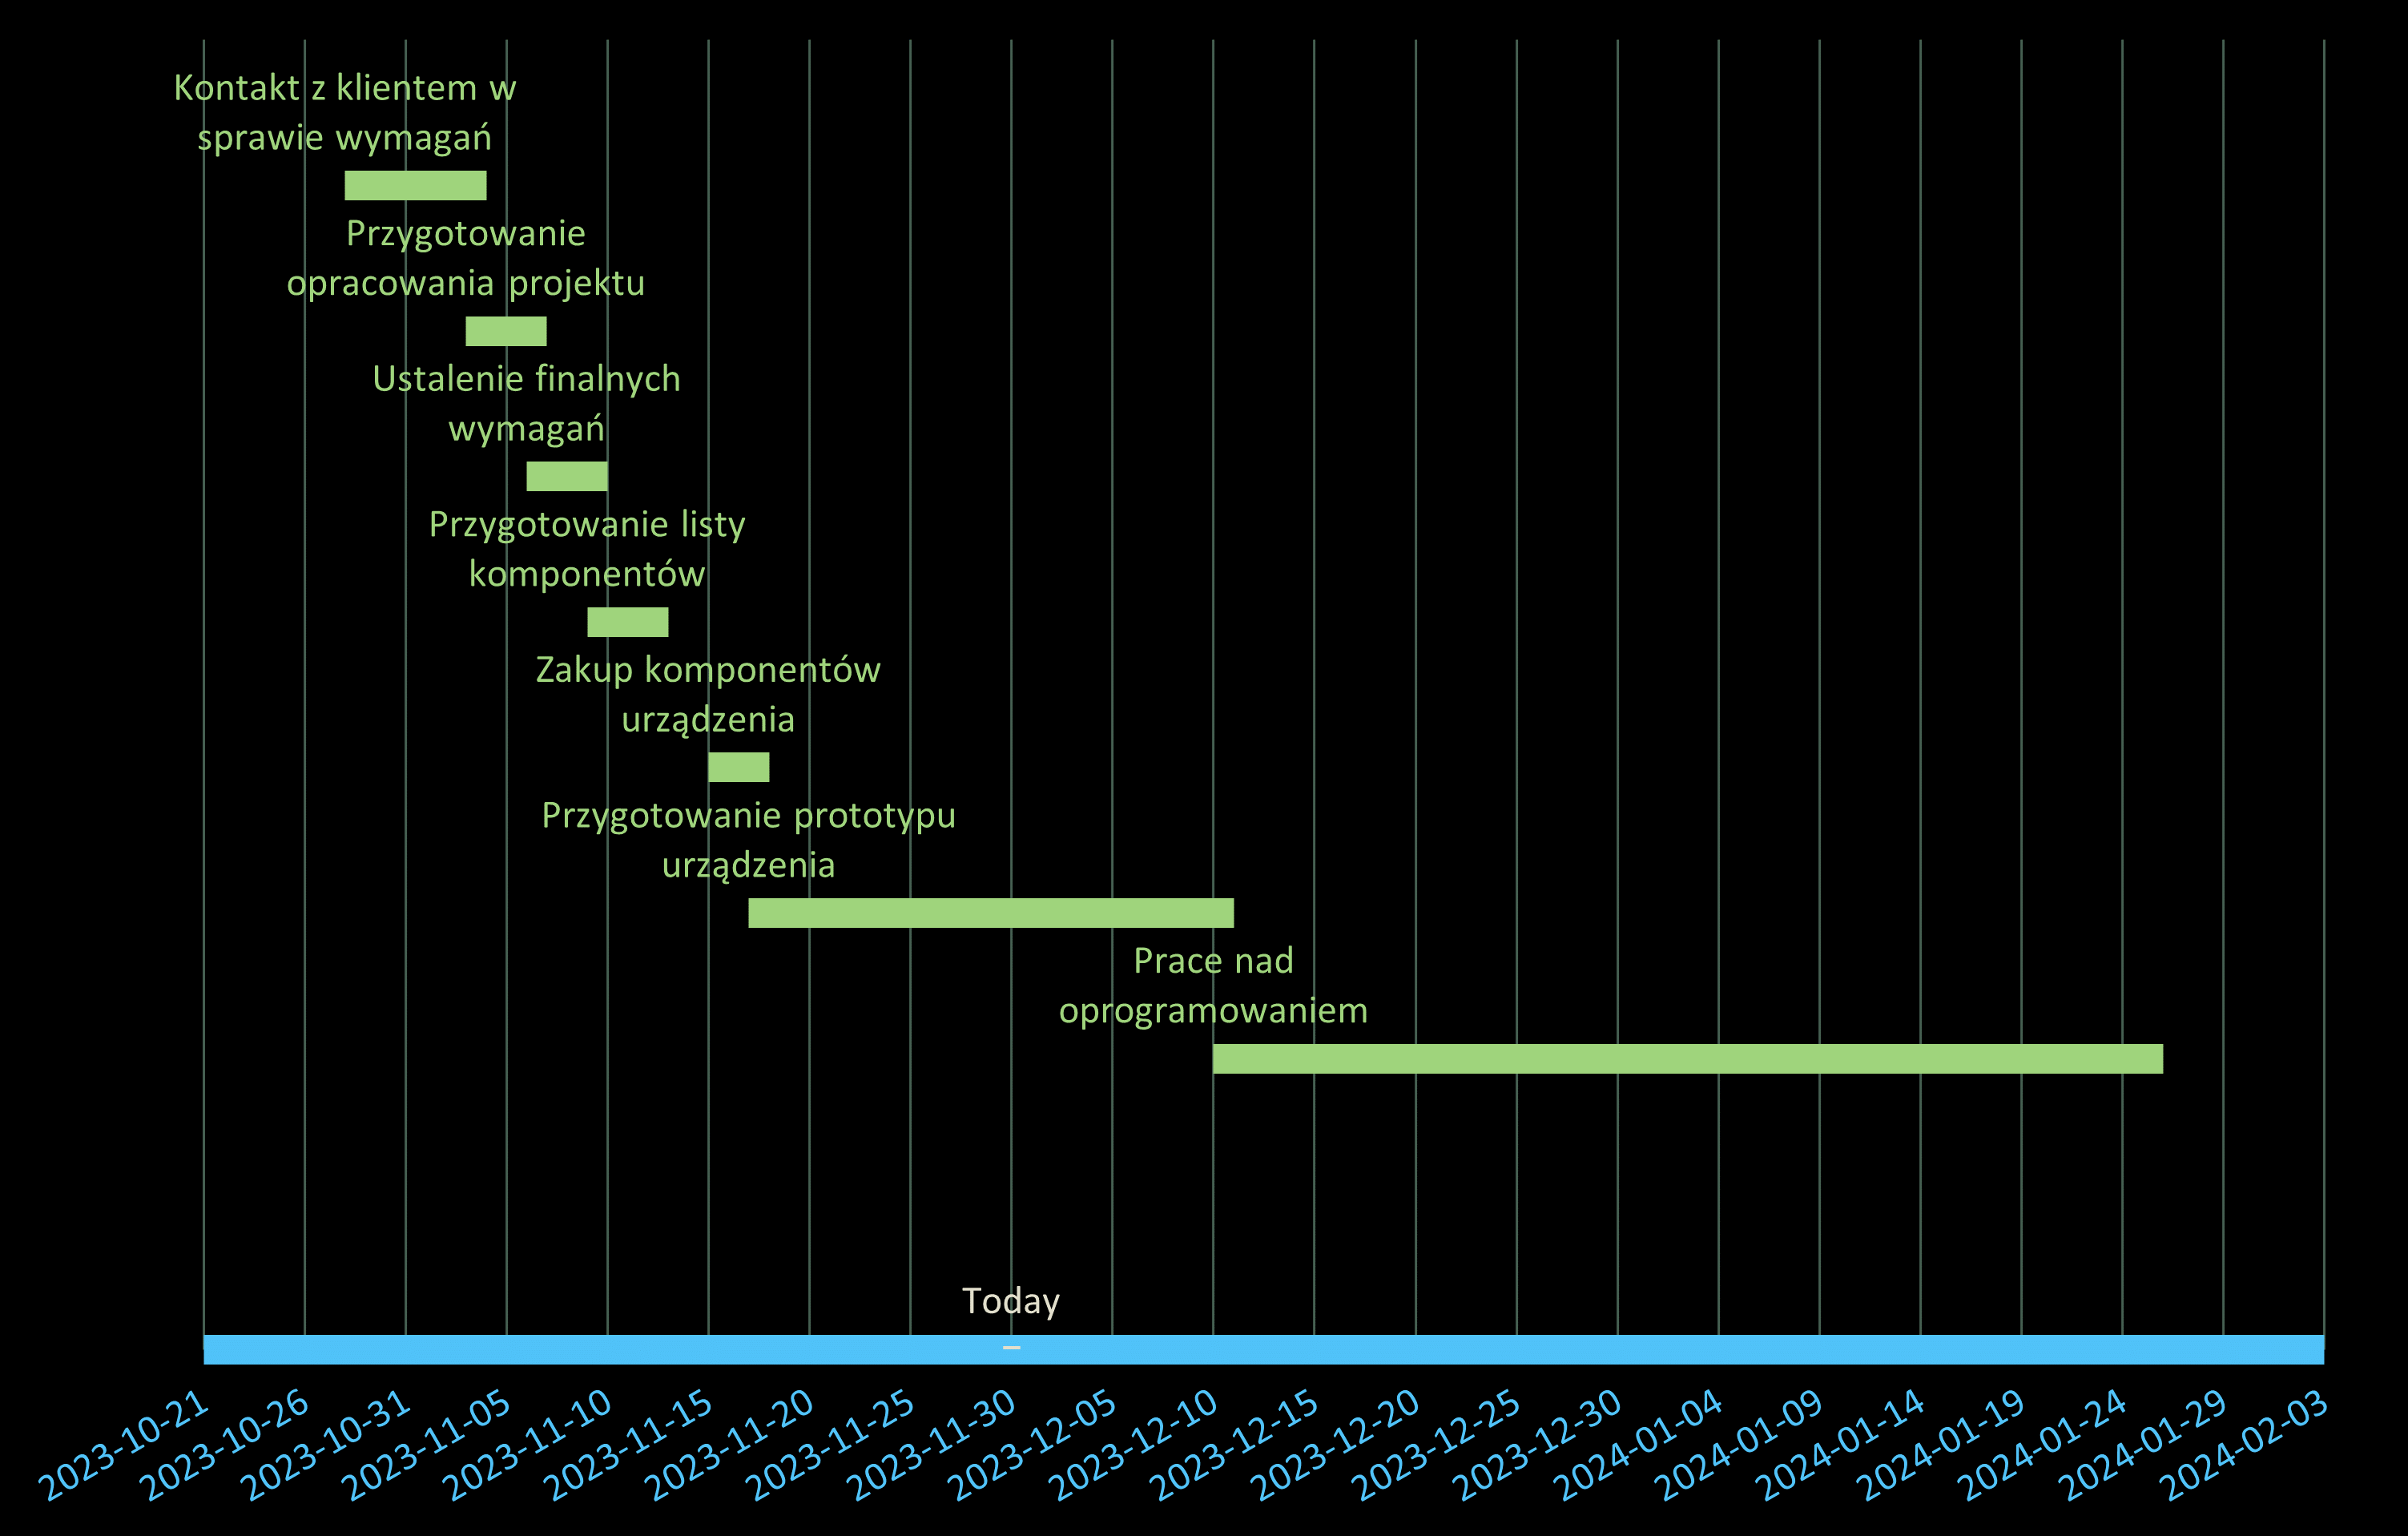
\includegraphics[width=\textwidth, center]{gantt.png}

\end{document}
